\section{Einf\"uhrung}

In diesem Projekt handelt es sich um das Erkennen von Durchgangswiderst\"anden
und deren Farbringe anhand eines gut beleuchteten  Fotos  einer Leiterplatine.
Das Foto wird senkrecht zur Platine aufgenommen und die Platine wird gerichtet
beleuchtet (Kamera-Blitz). Die Widerst\"ande sollten m\"oglichst flach auf der
Platine  liegen,   aufgestellte   Widerst\"ande   werden  nicht  erkannt.  Die
Widerst\"ande sollten weiter Blau-farbig sein.

\begin{figure}[H]
    \centering
    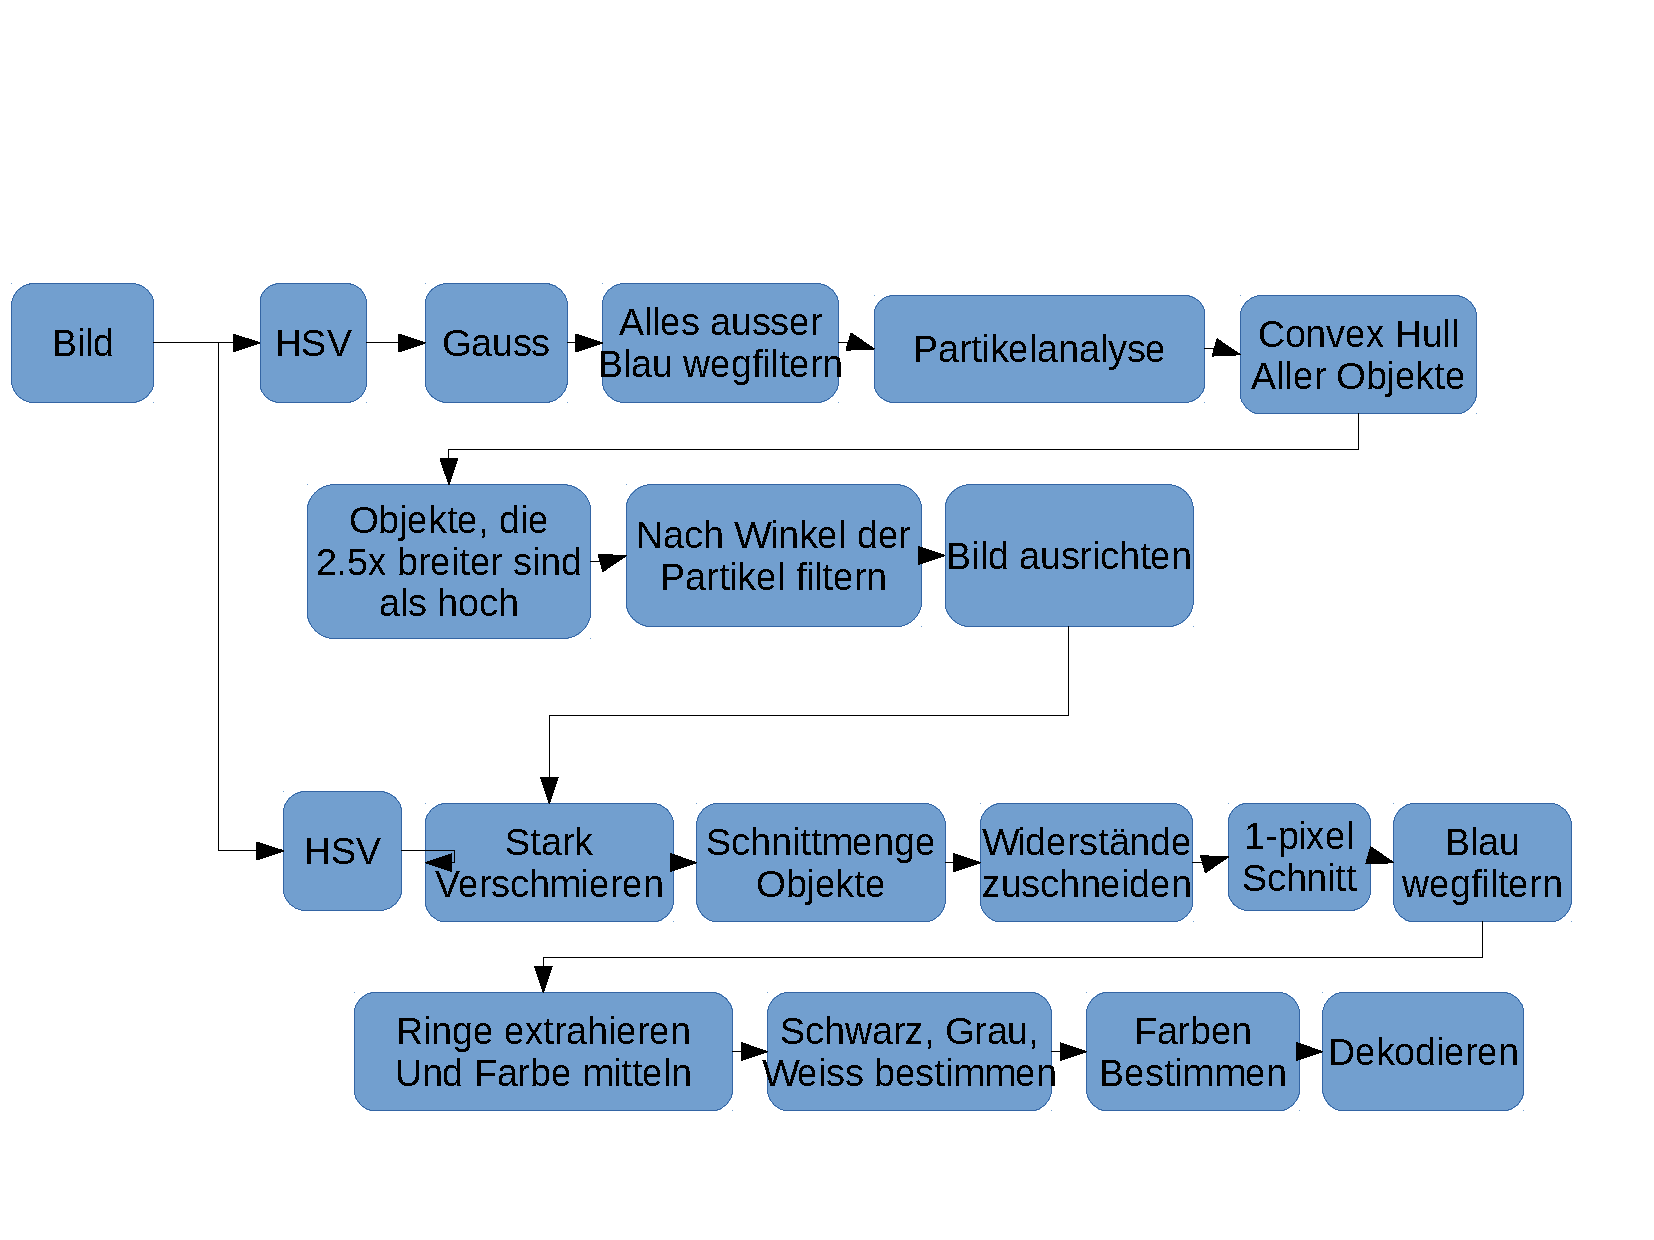
\includegraphics[width=\linewidth]{images/flow}
    \caption{\"Uberblick der Bildbearbeitung}
\end{figure}

